\documentclass[11pt]{article}
\usepackage[a4paper,margin=0.8in]{geometry}
\usepackage{hyperref}
\usepackage{enumitem}
\usepackage{titlesec}
\usepackage{xcolor}
\usepackage{fancyhdr}
\usepackage{tikz}
\usepackage{graphicx}
\usepackage{eso-pic}

\graphicspath{{../}}

\definecolor{kcpc-bg}{RGB}{250,250,250}
\definecolor{kcpc-text}{RGB}{20,20,20}
\definecolor{kcpc-muted}{RGB}{90,90,90}
\definecolor{kcpc-red}{RGB}{176,0,0}

\pagestyle{fancy}
\fancyhf{}
\lhead{\textcolor{kcpc-text}{\small\bfseries Reading List}}
\rhead{\textcolor{kcpc-muted}{\small Week 2}}
\cfoot{\textcolor{kcpc-muted}{\small KCPC}}
\renewcommand{\headrulewidth}{0.4pt}
\renewcommand{\headrule}{\hbox
to\headwidth{\color{kcpc-red}\leaders\hrule height \headrulewidth\hfill}}
\renewcommand{\footrulewidth}{0pt}
\setlength{\headheight}{28pt}

\AddToShipoutPictureBG{%
    \begin{tikzpicture}[remember picture,overlay]
        \node[opacity=0.035, at=(current page.center)]
        {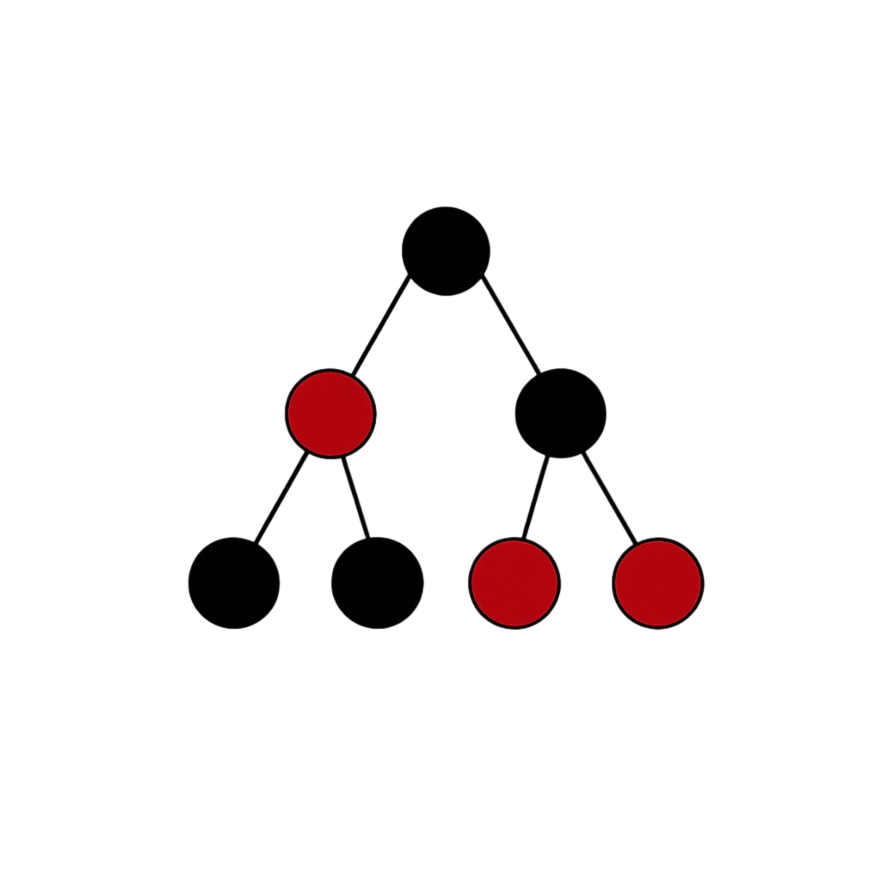
\includegraphics[width=0.38\paperwidth]{kcpc-logo.png}};
    \end{tikzpicture}%
}

\titleformat{\section}{\large\bfseries\color{kcpc-red}}{}{0pt}{}
\titlespacing*{\section}{0pt}{7pt}{2pt}
\setlist[itemize]{leftmargin=*, itemsep=0pt, topsep=1pt}
\setlength{\parindent}{0pt}
\newcommand{\bookentry}[2]{\textbf{#1}\par #2\par\vspace{7pt}}

\title{KCPC Week 2 Reading List\\Algorithmic Puzzle Strategies}
\author{}
\date{}

\begin{document}
\thispagestyle{fancy}

\begin{center}
    {\LARGE\bfseries KCPC Week 2 Reading List}\par
    \vspace{2pt}
    {\large Advanced Invariants, Heuristics, and Algorithmic Bridges}
\end{center}
\vspace{5pt}

\bookentry{The Art and Craft of Problem Solving Paul Zeitz (Wiley,
2007)}{The definitive guide to Zeitz heuristics: wishful thinking,
    symmetry, extreme principle, reduction. Chapters on invariants,
    colouring, and induction are exceptionally clear and directly
    relevant to both Week 1 and Week 2. The problems and solutions model
the kind of deep reasoning we practise.}

\bookentry{Problem-Solving Strategies Arthur Engel (Springer,
1998)}{A technique-centred encyclopaedia. The chapters on invariants,
    colouring proofs, and induction are the gold standard for
    mathematical problem solving. Many of the Week 2 exercises are drawn
from or inspired by Engel's examples.}

\bookentry{Mathematical Puzzles: A Connoisseur's Collection Peter
Winkler (A K Peters, 2004)}{Elegant puzzles that often require
    exactly the invariants, parity arguments, and induction techniques
    from the workshop. Winkler's solutions are concise and reveal the
core insight. Excellent for practising the transition from insight to proof.}

\bookentry{Algorithmic Puzzles Anany Levitin and Maria Levitin
(Oxford University Press, 2011)}{Bridges the gap between mathematical
    puzzles and algorithms. Organised by technique: state-space search,
    backtracking, greedy, divide-and-conquer, dynamic programming.
    Solutions discuss efficiency and implementation, making it ideal for
the algorithmic bridges in Week 2.}

\bookentry{Guide to Competitive Programming Antti Laaksonen
(Springer, 2017)}{A compact CP reference. Covers complexity, data
    structures, graph algorithms, greedy, DP, and more with short C++
    implementations. Use this to see how the mathematical ideas from Pair
    1 become standard CP algorithms in later pairs. The CSES problem set
(cses.fi) is a natural companion.}

\bookentry{Introduction to Algorithms: A Creative Approach Udi Manber
(Addison-Wesley, 1989)}{Organises algorithms around inductive proofs.
    Shows how a proof about smaller instances directly suggests a
    recursive or incremental algorithm. Connects Week 1 reasoning with
Week 2 bridges to DP, divide-and-conquer, and greedy algorithms.}

\bookentry{The Algorithm Design Manual Steven S. Skiena (Springer,
2020)}{A practical guide to recognising algorithmic problem types and
    choosing techniques. The "War Stories" show real modelling decisions.
    The catalogue of problems helps you map a puzzle to a known
algorithmic pattern. Complements the reduction heuristic from Week 2.}

\end{document}
